\documentclass[11pt,a4paper]{article}

% Image mode: pdf.
% Image paths stay relative. In PDF mode, place same-basename PDF conversions
% of the chapter SVG files in the assets/ directory beside this source.

\usepackage{iftex}
\ifPDFTeX
  \PackageError{handout}{This template requires XeTeX or Tectonic}{Compile with xelatex or tectonic.}
\fi

\usepackage[a4paper,top=18mm,bottom=20mm,left=20mm,right=20mm,headsep=6mm]{geometry}
\usepackage{fontspec}
\usepackage{xeCJK}
\usepackage{amsmath}
\usepackage{unicode-math}

% Font settings are intentionally visible in the generated .tex file.
% These defaults target the macOS machine used for the released PDF.
% Change the family names when compiling on another system.
\setmainfont{Songti TC}
\setsansfont{Heiti TC}
\setmonofont{Menlo}
\setCJKmainfont{Songti TC}
\setCJKsansfont{Heiti TC}
\setCJKmonofont{Heiti TC}
\setmathfont{STIX Two Math}
\XeTeXlinebreaklocale "zh"
\XeTeXlinebreakskip=0pt plus 1pt

\usepackage{xcolor}
\definecolor{HandoutBlue}{HTML}{215A91}
\definecolor{HandoutBlueLight}{HTML}{EEF5FC}
\definecolor{HandoutGreen}{HTML}{39715A}
\definecolor{HandoutGreenLight}{HTML}{EFF8F3}
\definecolor{HandoutGold}{HTML}{8A641C}
\definecolor{HandoutGoldLight}{HTML}{FFF8E8}
\definecolor{HandoutInk}{HTML}{253142}
\definecolor{HandoutMuted}{HTML}{667085}

\usepackage{graphicx}
\makeatletter
% Pandoc 3 emits an accessibility `alt` key for raster/PDF images. Older
% graphicx releases do not know that key, so accept it without changing layout.
\@ifundefined{KV@Gin@alt}{\define@key{Gin}{alt}{}}{}
\newsavebox\pandoc@box
\newcommand*\pandocbounded[1]{%
  \sbox\pandoc@box{#1}%
  \Gscale@div\@tempa{\textheight}{\dimexpr\ht\pandoc@box+\dp\pandoc@box\relax}%
  \Gscale@div\@tempb{\linewidth}{\wd\pandoc@box}%
  \ifdim\@tempb\p@<\@tempa\p@\let\@tempa\@tempb\fi
  \ifdim\@tempa\p@<\p@\scalebox{\@tempa}{\usebox\pandoc@box}%
  \else\usebox{\pandoc@box}%
  \fi
}
\makeatother
\usepackage{float}
\floatplacement{figure}{H}
% Pandoc uses LTcaptype=none for uncaptioned longtables. The caption package
% expects that name to exist as a counter even though it is never displayed.
\newcounter{none}
\usepackage{caption}
\captionsetup[figure]{labelformat=empty,labelsep=none,font=small}

\usepackage{booktabs,longtable,array,calc}
\usepackage{etoolbox}
\makeatletter
\patchcmd\longtable{\par}{\if@noskipsec\mbox{}\fi\par}{}{}
\makeatother

\usepackage[most]{tcolorbox}
\tcbuselibrary{breakable,skins}
\newtcolorbox{HandoutLearningMap}{
  enhanced,breakable,colback=HandoutBlueLight,colframe=HandoutBlue,
  boxrule=0.8pt,arc=1.5mm,left=3mm,right=3mm,top=2mm,bottom=2mm,
  before skip=8pt,after skip=10pt
}
\newtcolorbox{HandoutWorkedExample}{
  enhanced,breakable,colback=HandoutGreenLight,colframe=HandoutGreen,
  boxrule=0.65pt,arc=1.5mm,left=3mm,right=3mm,top=2mm,bottom=2mm,
  before skip=8pt,after skip=10pt
}
\newtcolorbox{HandoutSelfCheck}{
  enhanced,breakable,colback=HandoutGoldLight,colframe=HandoutGold,
  boxrule=0.65pt,arc=1.5mm,left=3mm,right=3mm,top=2mm,bottom=2mm,
  before skip=8pt,after skip=10pt
}

\usepackage{titlesec}
\titleformat{\section}{\sffamily\bfseries\Large\color{HandoutBlue}}{}{0pt}{}
\titleformat{\subsection}{\sffamily\bfseries\large\color{HandoutInk}}{}{0pt}{}
\titleformat{\subsubsection}{\sffamily\bfseries\normalsize\color{HandoutInk}}{}{0pt}{}
\titlespacing*{\section}{0pt}{1.4em}{0.55em}
\titlespacing*{\subsection}{0pt}{1.15em}{0.45em}
\titlespacing*{\subsubsection}{0pt}{0.9em}{0.35em}
\setcounter{secnumdepth}{-\maxdimen}

\usepackage{hyperref}
\usepackage{bookmark}
\IfFileExists{xurl.sty}{\usepackage{xurl}}{}
\urlstyle{same}
\hypersetup{
  colorlinks=true,
  linkcolor=HandoutBlue,
  urlcolor=HandoutBlue,
  citecolor=HandoutBlue,
  pdftitle={數A4-3 條件機率與貝氏定理},
  pdfsubject={數學},
  pdfcreator={Pandoc with the HighSchooContent LaTeX template}
}

\setlength{\parindent}{0pt}
\setlength{\parskip}{0.55em plus 0.15em minus 0.1em}
\setlength{\emergencystretch}{3em}
\setlength{\LTpre}{0.5em}
\setlength{\LTpost}{0.5em}
\renewcommand{\arraystretch}{1.18}
\providecommand{\tightlist}{%
  \setlength{\itemsep}{0pt}\setlength{\parskip}{0pt}}
\pagestyle{plain}


\begin{document}

\begin{tcolorbox}[
  enhanced,colback=white,colframe=HandoutBlue,boxrule=1.1pt,arc=2mm,
  borderline west={3pt}{0pt}{HandoutBlue},left=5mm,right=4mm,top=4mm,bottom=4mm
]
{\sffamily\small\bfseries\color{HandoutBlue}學生講義}\par
{\sffamily\bfseries\LARGE\color{HandoutInk}數A4-3 條件機率與貝氏定理}\par
\vspace{0.35em}{\large 用已知資訊縮小樣本空間，判斷事件是否獨立，並由新證據更新原先機率}\par
\vspace{0.45em}{\small\color{HandoutMuted}%
科目：數學
\quad 課程：普通高中數學A 第四冊
\quad 版本：學生版｜核心＋理解
\quad 校訂：2026-08-29
}\par
\vspace{0.25em}{\small\color{HandoutMuted}範圍：機率性質、條件機率、獨立事件、乘法法則、全機率公式、貝氏定理、主觀與客觀機率}\par
\end{tcolorbox}


\section{本章核心問題}\label{ux672cux7ae0ux6838ux5fc3ux554fux984c}

同一件事在加入資訊後，機率可能改變。快篩陽性的人確實帶原的機率、看到瑕疵品後推測來源工廠、已知前兩局結果後估計贏得系列賽的機率，都需要先說清楚「目前已知什麼」。

本章建立六個相連的工具：

\begin{enumerate}
\def\labelenumi{\arabic{enumi}.}
\tightlist
\item
  用事件運算整理所有可能結果；
\item
  用條件機率把已知事件當成新的樣本空間；
\item
  用乘積條件判斷資訊是否改變另一事件；
\item
  用乘法法則計算連續發生的路徑；
\item
  用全機率公式合併不同來源；
\item
  用貝氏定理在看見結果後更新來源機率。
\end{enumerate}

品管、醫療檢驗、垃圾郵件過濾、氣象預報與風險評估都使用同一個結構：先有來源比例，再有各來源產生證據的機率，最後根據實際觀察重新分配機率。

\section{1. 機率性質與條件機率}\label{ux6a5fux7387ux6027ux8ceaux8207ux689dux4ef6ux6a5fux7387}

\subsection{1.1 事件運算與機率性質}\label{ux4e8bux4ef6ux904bux7b97ux8207ux6a5fux7387ux6027ux8cea}

樣本空間 \(S\) 是一次隨機試驗所有可能結果的集合；事件 \(A\) 是 \(S\) 的子集合。機率函數滿足

\[
0\le P(A)\le1,
\qquad
P(S)=1,
\qquad
P(\emptyset)=0.
\]

\(A'\) 表示 \(A\) 的餘事件，因此

\[
P(A')=1-P(A).
\]

兩事件聯集的加法公式為

\[
\boxed{P(A\cup B)=P(A)+P(B)-P(A\cap B)}.
\]

推理來自重複計數：\(P(A)+P(B)\) 把交集 \(A\cap B\) 算了兩次，減去一次後，每個結果恰好計一次。當 \(A,B\) 互斥時，\(A\cap B=\emptyset\)，公式化為 \(P(A\cup B)=P(A)+P(B)\)。

\begin{HandoutWorkedExample}

\subsection{完整示範｜聯集、交集與都未發生}\label{ux5b8cux6574ux793aux7bc4ux806fux96c6ux4ea4ux96c6ux8207ux90fdux672aux767cux751f}

某校學生使用公車通學的比例為 \(0.62\)，使用捷運通學的比例為 \(0.47\)，兩者都使用的比例為 \(0.30\)。求至少使用其中一種交通工具，以及兩種都未使用的比例。

令 \(A\) 為使用公車、\(B\) 為使用捷運。至少使用一種就是 \(A\cup B\)：

\[
P(A\cup B)=0.62+0.47-0.30=0.79.
\]

兩種都未使用是 \((A\cup B)'\)：

\[
P((A\cup B)')=1-0.79=0.21.
\]

答案為 \(\boxed{0.79}\) 與 \(\boxed{0.21}\)，兩者相加為 \(1\)。

\end{HandoutWorkedExample}

\begin{HandoutWorkedExample}

\subsection{完整示範｜由邊際機率判斷交集範圍}\label{ux5b8cux6574ux793aux7bc4ux7531ux908aux969bux6a5fux7387ux5224ux65b7ux4ea4ux96c6ux7bc4ux570d}

已知 \(P(A)=0.55\)、\(P(B)=0.70\)。求 \(P(A\cap B)\) 的可能範圍。

交集最多等於較小事件的機率：

\[
P(A\cap B)\le\min(0.55,0.70)=0.55.
\]

又因 \(P(A\cup B)\le1\)，

\[
0.55+0.70-P(A\cap B)\le1,
\]

所以 \(P(A\cap B)\ge0.25\)。因此

\[
\boxed{0.25\le P(A\cap B)\le0.55}.
\]

下界代表兩事件合起來剛好覆蓋全部；上界代表 \(A\) 完全包含在 \(B\) 中。

\end{HandoutWorkedExample}

\subsection{1.2 條件機率：已知資訊決定分母}\label{ux689dux4ef6ux6a5fux7387ux5df2ux77e5ux8cc7ux8a0aux6c7aux5b9aux5206ux6bcd}

在事件 \(A\) 已發生的條件下，只保留 \(A\) 內的結果。事件 \(B\) 在這個新樣本空間中的比例為

\[
\boxed{
P(B\mid A)=\frac{P(A\cap B)}{P(A)}
},
\qquad P(A)>0.
\]

分子是同時符合 \(A\) 與 \(B\) 的機率；分母是目前所有仍可能的 \(A\)。條件順序會決定分母，因此 \(P(B\mid A)\) 與 \(P(A\mid B)\) 通常不同。

\begin{figure}
\centering
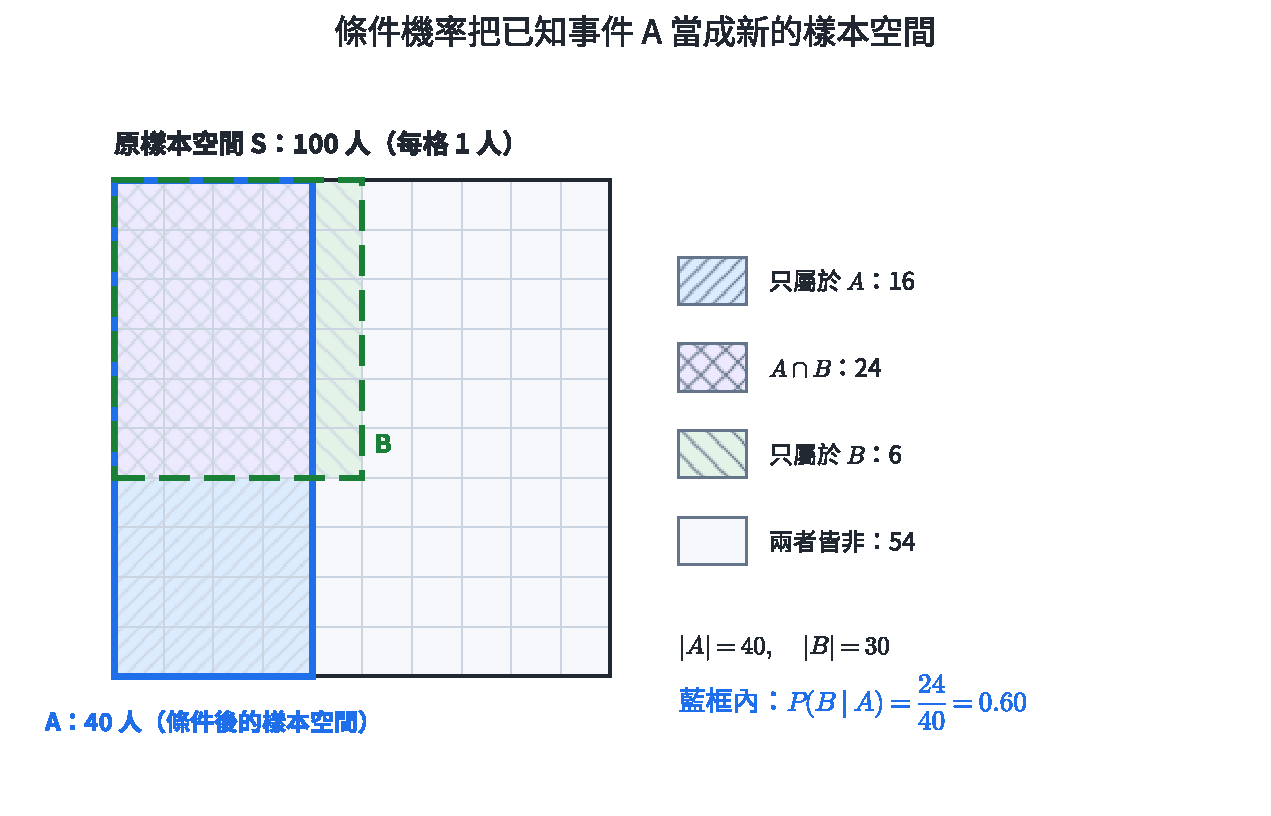
\includegraphics[width=0.88\linewidth,height=\textheight,keepaspectratio,alt={圖 1｜給定事件 A 後，樣本空間縮成 A；交集在 A 內所占比例就是條件機率。}]{assets/數A4-3-條件樣本空間.pdf}
\caption{圖 1｜給定事件 A 後，樣本空間縮成 A；交集在 A 內所占比例就是條件機率。}
\end{figure}

\begin{HandoutWorkedExample}

\subsection{完整示範｜雙向表中的兩個條件方向}\label{ux5b8cux6574ux793aux7bc4ux96d9ux5411ux8868ux4e2dux7684ux5169ux500bux689dux4ef6ux65b9ux5411}

某群體共 \(100\) 人，資料如下：

{\def\LTcaptype{none} % do not increment counter
\begin{longtable}[]{@{}lrrr@{}}
\toprule\noalign{}
& \(B\) & \(B'\) & 合計 \\
\midrule\noalign{}
\endhead
\bottomrule\noalign{}
\endlastfoot
\(A\) & 24 & 16 & 40 \\
\(A'\) & 6 & 54 & 60 \\
合計 & 30 & 70 & 100 \\
\end{longtable}
}

已知 \(A\) 時，分母取 \(A\) 列的 \(40\) 人：

\[
P(B\mid A)=\frac{24}{40}=0.60.
\]

已知 \(B\) 時，分母取 \(B\) 欄的 \(30\) 人：

\[
P(A\mid B)=\frac{24}{30}=0.80.
\]

兩式共用同一個交集人數 \(24\)，條件方向使分母不同。

\end{HandoutWorkedExample}

\begin{figure}
\centering
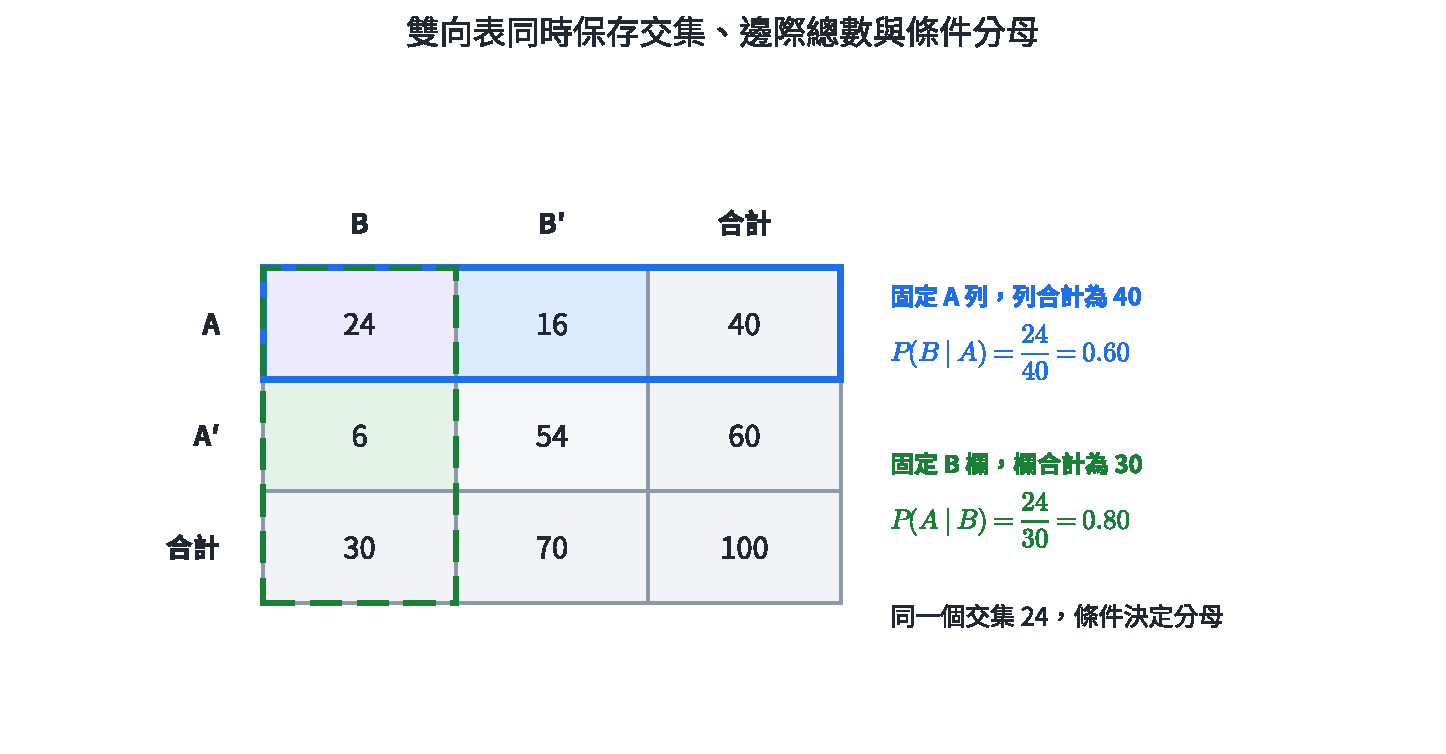
\includegraphics[width=0.88\linewidth,height=\textheight,keepaspectratio,alt={圖 2｜雙向表的列、欄總數就是兩種條件方向的分母。}]{assets/數A4-3-雙向條件表.pdf}
\caption{圖 2｜雙向表的列、欄總數就是兩種條件方向的分母。}
\end{figure}

\begin{HandoutWorkedExample}

\subsection{完整示範｜在點數和已知後重新列樣本}\label{ux5b8cux6574ux793aux7bc4ux5728ux9edeux6578ux548cux5df2ux77e5ux5f8cux91cdux65b0ux5217ux6a23ux672c}

擲兩顆公正骰子，已知點數和為 \(8\)，求第一顆點數至少為 \(3\) 的機率。

在和為 \(8\) 的條件下，等可能的有序結果為

\[
(2,6),(3,5),(4,4),(5,3),(6,2).
\]

其中第一顆至少為 \(3\) 的結果有後四個，因此

\[
\boxed{P(\text{第一顆}\ge3\mid\text{和為 }8)=\frac45}.
\]

條件已把原本 \(36\) 個結果縮成 \(5\) 個；計數只在這 \(5\) 個結果中進行。

\end{HandoutWorkedExample}

\begin{HandoutWorkedExample}

\subsection{完整示範｜用機率式反轉條件方向}\label{ux5b8cux6574ux793aux7bc4ux7528ux6a5fux7387ux5f0fux53cdux8f49ux689dux4ef6ux65b9ux5411}

已知

\[
P(A)=0.40,
\qquad
P(B\mid A)=0.75,
\qquad
P(B)=0.50.
\]

先由條件機率求交集：

\[
P(A\cap B)=P(A)P(B\mid A)=0.40\times0.75=0.30.
\]

再換分母：

\[
P(A\mid B)=\frac{P(A\cap B)}{P(B)}
=\frac{0.30}{0.50}
=\boxed{0.60}.
\]

\end{HandoutWorkedExample}

\begin{HandoutSelfCheck}

\subsection{分節練習｜事件與條件機率}\label{ux5206ux7bc0ux7df4ux7fd2ux4e8bux4ef6ux8207ux689dux4ef6ux6a5fux7387}

\begin{enumerate}
\def\labelenumi{\arabic{enumi}.}
\tightlist
\item
  已知 \(P(A)=0.58\)、\(P(B)=0.37\)、\(P(A\cap B)=0.21\)，求 \(P(A\cup B)\) 與 \(P(A'\cap B')\)。
\item
  已知 \(P(A)=0.45\)、\(P(B)=0.60\)、\(P(A\cup B)=0.78\)，求 \(P(A\cap B)\)。
\item
  某次測驗共 \(160\) 人，數學及格 \(100\) 人、英文及格 \(80\) 人、兩科皆及格 \(65\) 人。求 \(P(E\mid M)\)、\(P(M\mid E)\) 與 \(P(E'\mid M)\)。
\item
  擲兩顆公正骰子，已知點數和為 \(9\)，求第一顆點數大於第二顆的機率。
\item
  從一副 \(52\) 張撲克牌任取一張，已知抽到的是 J、Q 或 K，求它是 Q 的機率。
\item
  已知 \(P(A)=0.40\)、\(P(B\mid A)=0.75\)、\(P(B)=0.50\)，求 \(P(A\cap B)\) 與 \(P(A\mid B)\)。
\end{enumerate}

\textbf{解答}

\begin{enumerate}
\def\labelenumi{\arabic{enumi}.}
\tightlist
\item
  \(P(A\cup B)=0.58+0.37-0.21=\boxed{0.74}\)；\(P(A'\cap B')=1-0.74=\boxed{0.26}\)。
\item
  \(P(A\cap B)=0.45+0.60-0.78=\boxed{0.27}\)。
\item
  \(P(E\mid M)=65/100=\boxed{0.65}\)；\(P(M\mid E)=65/80=\boxed{0.8125}\)；\(P(E'\mid M)=35/100=\boxed{0.35}\)。
\item
  和為 \(9\) 的結果為 \((3,6),(4,5),(5,4),(6,3)\)；後兩個符合，答案 \(\boxed{1/2}\)。
\item
  J、Q、K 共 \(12\) 張，其中 Q 有 \(4\) 張，答案 \(\boxed{1/3}\)。
\item
  \(P(A\cap B)=0.40(0.75)=\boxed{0.30}\)；\(P(A\mid B)=0.30/0.50=\boxed{0.60}\)。
\end{enumerate}

\end{HandoutSelfCheck}

\section{2. 獨立事件}\label{ux7368ux7acbux4e8bux4ef6}

\subsection{2.1 定義與資訊意義}\label{ux5b9aux7fa9ux8207ux8cc7ux8a0aux610fux7fa9}

若事件 \(A\) 的發生不改變事件 \(B\) 的機率，則

\[
P(B\mid A)=P(B).
\]

代入條件機率定義可得

\[
\boxed{P(A\cap B)=P(A)P(B)}.
\]

這個乘積式對 \(A,B\) 對稱，且在零機率事件也可使用，因此採為兩事件獨立的正式定義。

互斥描述「不能同時發生」，獨立描述「知道一件事後，另一件事的比例維持不變」。兩個正機率事件若互斥，交集機率為 \(0\)，而乘積為正，因此不會獨立。

\begin{figure}
\centering
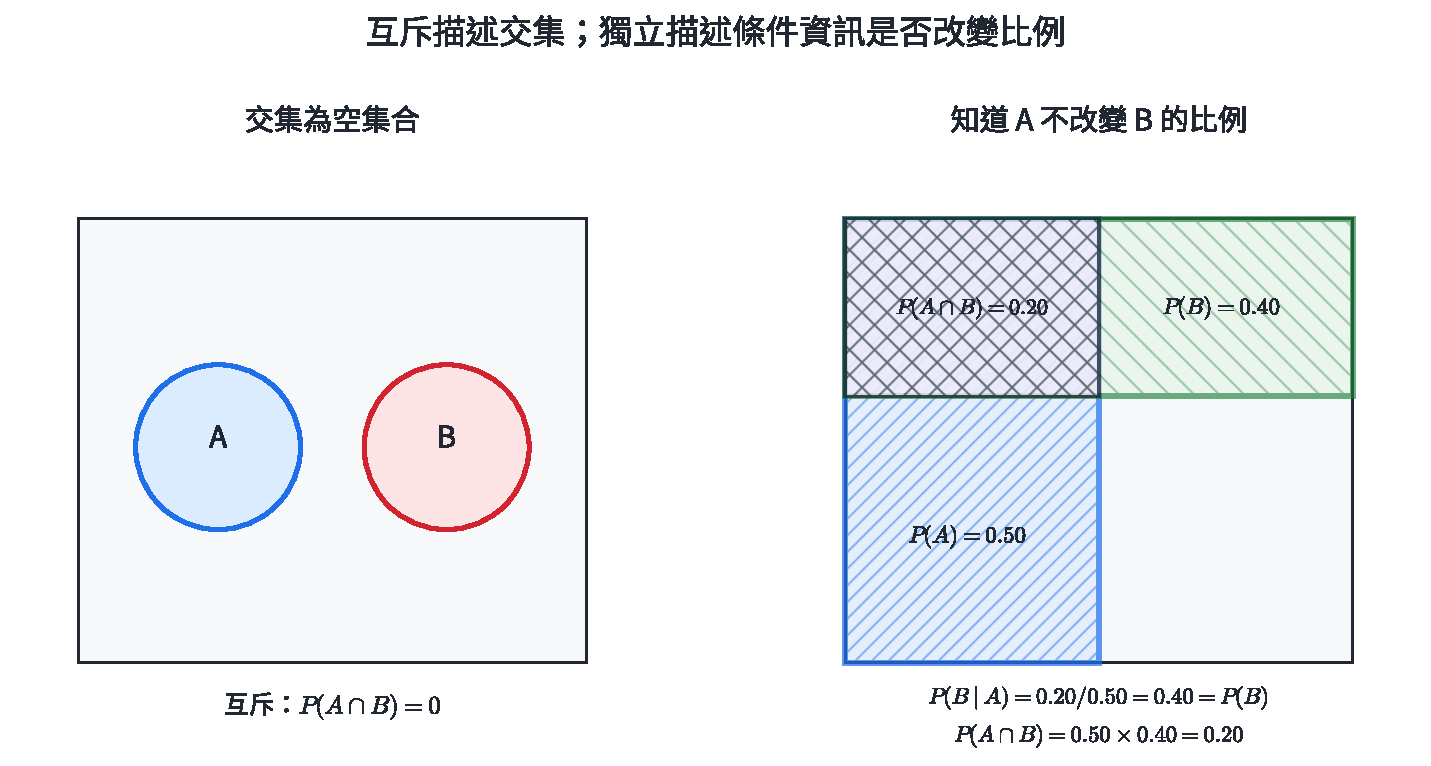
\includegraphics[width=0.9\linewidth,height=\textheight,keepaspectratio,alt={圖 3｜互斥由交集為零描述；獨立由交集面積等於兩個邊際比例的乘積描述。}]{assets/數A4-3-互斥與獨立.pdf}
\caption{圖 3｜互斥由交集為零描述；獨立由交集面積等於兩個邊際比例的乘積描述。}
\end{figure}

\begin{HandoutWorkedExample}

\subsection{完整示範｜用乘積式判斷獨立}\label{ux5b8cux6574ux793aux7bc4ux7528ux4e58ux7a4dux5f0fux5224ux65b7ux7368ux7acb}

擲一顆公正骰子。令

\[
A=\{1,3,5\},
\qquad
B=\{1,2\}.
\]

\[
P(A)=\frac12,
\qquad
P(B)=\frac13,
\qquad
P(A\cap B)=P(\{1\})=\frac16.
\]

因為

\[
P(A\cap B)=\frac16=\frac12\cdot\frac13=P(A)P(B),
\]

所以 \(A,B\) 獨立。這不代表兩事件沒有交集；結果 \(1\) 同時屬於兩者。

\end{HandoutWorkedExample}

\begin{HandoutWorkedExample}

\subsection{完整示範｜互斥事件的資訊效果}\label{ux5b8cux6574ux793aux7bc4ux4e92ux65a5ux4e8bux4ef6ux7684ux8cc7ux8a0aux6548ux679c}

同一顆骰子中，令 \(C=\{1,3,5\}\)、\(D=\{2,4,6\}\)。兩事件互斥，

\[
P(C\cap D)=0.
\]

但

\[
P(C)P(D)=\frac12\cdot\frac12=\frac14.
\]

所以 \(C,D\) 不獨立。若已知 \(C\) 發生，\(D\) 的條件機率由原本 \(1/2\) 變成 \(0\)；這正是強烈的資訊影響。

\end{HandoutWorkedExample}

\subsection{2.2 餘事件與多事件獨立}\label{ux9918ux4e8bux4ef6ux8207ux591aux4e8bux4ef6ux7368ux7acb}

若 \(A,B\) 獨立，則

\[
\begin{aligned}
P(A'\cap B)
&=P(B)-P(A\cap B)\\
&=P(B)-P(A)P(B)\\
&=(1-P(A))P(B)\\
&=P(A')P(B).
\end{aligned}
\]

因此 \(A',B\) 也獨立；同理 \(A,B'\) 與 \(A',B'\) 都獨立。

三事件 \(A,B,C\) 共同獨立時，需同時滿足三個兩兩乘積式與三重乘積式：

\[
\begin{gathered}
P(A\cap B)=P(A)P(B),\\
P(A\cap C)=P(A)P(C),\\
P(B\cap C)=P(B)P(C),\\
P(A\cap B\cap C)=P(A)P(B)P(C).
\end{gathered}
\]

\begin{HandoutWorkedExample}

\subsection{完整示範｜兩個獨立設備的系統可靠度}\label{ux5b8cux6574ux793aux7bc4ux5169ux500bux7368ux7acbux8a2dux5099ux7684ux7cfbux7d71ux53efux9760ux5ea6}

兩個感測器獨立運作，正常率分別為 \(0.92\) 與 \(0.85\)。

兩者都正常的機率為

\[
0.92\times0.85=\boxed{0.782}.
\]

至少一個正常，可由「兩個都失效」的餘事件求得：

\[
1-(1-0.92)(1-0.85)
=1-0.08\times0.15
=\boxed{0.988}.
\]

並聯系統只需一個元件正常時，餘事件法直接對應系統完全失效的條件。

\end{HandoutWorkedExample}

\begin{HandoutWorkedExample}

\subsection{完整示範｜兩兩獨立仍需檢查三重交集}\label{ux5b8cux6574ux793aux7bc4ux5169ux5169ux7368ux7acbux4ecdux9700ux6aa2ux67e5ux4e09ux91cdux4ea4ux96c6}

擲一枚均勻硬幣兩次，樣本空間為

\[
S=\{HH,HT,TH,TT\}.
\]

令 \(A\) 為第一次是正面、\(B\) 為第二次是正面、\(C\) 為兩次相同。三事件機率都為 \(1/2\)。

任兩事件的交集都只有一個結果，機率為 \(1/4=(1/2)(1/2)\)，所以三對事件兩兩獨立。但

\[
A\cap B\cap C=\{HH\},
\]

\[
P(A\cap B\cap C)=\frac14
\ne
\frac12\cdot\frac12\cdot\frac12=\frac18.
\]

因此三事件沒有共同獨立。兩兩檢查只確認二階關係，三重交集仍需另行驗證。

\end{HandoutWorkedExample}

\begin{HandoutWorkedExample}

\subsection{完整示範｜由獨立性補完雙向表}\label{ux5b8cux6574ux793aux7bc4ux7531ux7368ux7acbux6027ux88dcux5b8cux96d9ux5411ux8868}

某群體有 \(200\) 人，事件 \(A\) 有 \(120\) 人，事件 \(B\) 有 \(80\) 人，且 \(A,B\) 獨立。求四格人數。

\[
P(A\cap B)=P(A)P(B)
=\frac{120}{200}\cdot\frac{80}{200}
=0.24.
\]

交集人數為 \(200(0.24)=48\)。其餘三格依列、欄總數相減：

{\def\LTcaptype{none} % do not increment counter
\begin{longtable}[]{@{}lrrr@{}}
\toprule\noalign{}
& \(B\) & \(B'\) & 合計 \\
\midrule\noalign{}
\endhead
\bottomrule\noalign{}
\endlastfoot
\(A\) & 48 & 72 & 120 \\
\(A'\) & 32 & 48 & 80 \\
合計 & 80 & 120 & 200 \\
\end{longtable}
}

每一列中 \(B\) 所占比例都為 \(0.40\)，直接呈現獨立的資訊意義。

\end{HandoutWorkedExample}

\begin{HandoutSelfCheck}

\subsection{分節練習｜獨立事件}\label{ux5206ux7bc0ux7df4ux7fd2ux7368ux7acbux4e8bux4ef6}

\begin{enumerate}
\def\labelenumi{\arabic{enumi}.}
\tightlist
\item
  已知 \(P(A)=0.40\)、\(P(B)=0.25\)、\(P(A\cap B)=0.10\)，判斷 \(A,B\) 是否獨立。
\item
  \(A,B\) 互斥，且 \(P(A)=0.40\)、\(P(B)=0.30\)。判斷兩事件是否獨立。
\item
  \(A,B\) 獨立，\(P(A)=0.70\)、\(P(B)=0.60\)。求兩者都發生、都未發生、恰一個發生、至少一個發生的機率。
\item
  三個設備獨立正常，正常率依序為 \(0.80,0.70,0.90\)。求全部正常、全部失效、至少一個正常、恰兩個正常的機率。
\item
  在兩次擲硬幣模型中，令 \(A\) 為第一次正面、\(B\) 為第二次正面、\(C\) 為兩次相同。驗證任兩事件獨立，並判斷三事件是否共同獨立。
\item
  某群體 \(200\) 人中，\(A\) 有 \(120\) 人、\(B\) 有 \(80\) 人，且 \(A,B\) 獨立。完成四格表。
\end{enumerate}

\textbf{解答}

\begin{enumerate}
\def\labelenumi{\arabic{enumi}.}
\tightlist
\item
  \(P(A)P(B)=0.40(0.25)=0.10=P(A\cap B)\)，所以 \(\boxed{\text{獨立}}\)。
\item
  \(P(A\cap B)=0\)，而 \(P(A)P(B)=0.12\)，所以 \(\boxed{\text{不獨立}}\)。
\item
  都發生 \(\boxed{0.42}\)；都未發生 \(0.30(0.40)=\boxed{0.12}\)；恰一個 \(0.70(0.40)+0.30(0.60)=\boxed{0.46}\)；至少一個 \(1-0.12=\boxed{0.88}\)。
\item
  全部正常 \(0.8(0.7)(0.9)=\boxed{0.504}\)；全部失效 \(0.2(0.3)(0.1)=\boxed{0.006}\)；至少一個正常 \(\boxed{0.994}\)；恰兩個正常 \(0.8(0.7)(0.1)+0.8(0.3)(0.9)+0.2(0.7)(0.9)=\boxed{0.398}\)。
\item
  三對交集機率都是 \(1/4=(1/2)(1/2)\)；三重交集為 \(1/4\)，而三個邊際機率乘積為 \(1/8\)，所以兩兩獨立但未共同獨立。
\item
  四格依序為 \(A\cap B=48\)、\(A\cap B'=72\)、\(A'\cap B=32\)、\(A'\cap B'=48\)。
\end{enumerate}

\end{HandoutSelfCheck}

\section{3. 條件機率的乘法法則與連續路徑}\label{ux689dux4ef6ux6a5fux7387ux7684ux4e58ux6cd5ux6cd5ux5247ux8207ux9023ux7e8cux8defux5f91}

\subsection{3.1 兩事件與多事件的乘法法則}\label{ux5169ux4e8bux4ef6ux8207ux591aux4e8bux4ef6ux7684ux4e58ux6cd5ux6cd5ux5247}

由條件機率定義移項：

\[
\boxed{P(A\cap B)=P(A)P(B\mid A)}.
\]

對三事件依序套用：

\[
\boxed{
P(A\cap B\cap C)
=P(A)P(B\mid A)P(C\mid A\cap B)
}.
\]

每一因子都是「走到目前節點後，下一步沿指定分支前進」的條件機率。樹狀圖的一條完整路徑用乘法；多條互斥路徑通往同一結果時再相加。

\begin{figure}
\centering
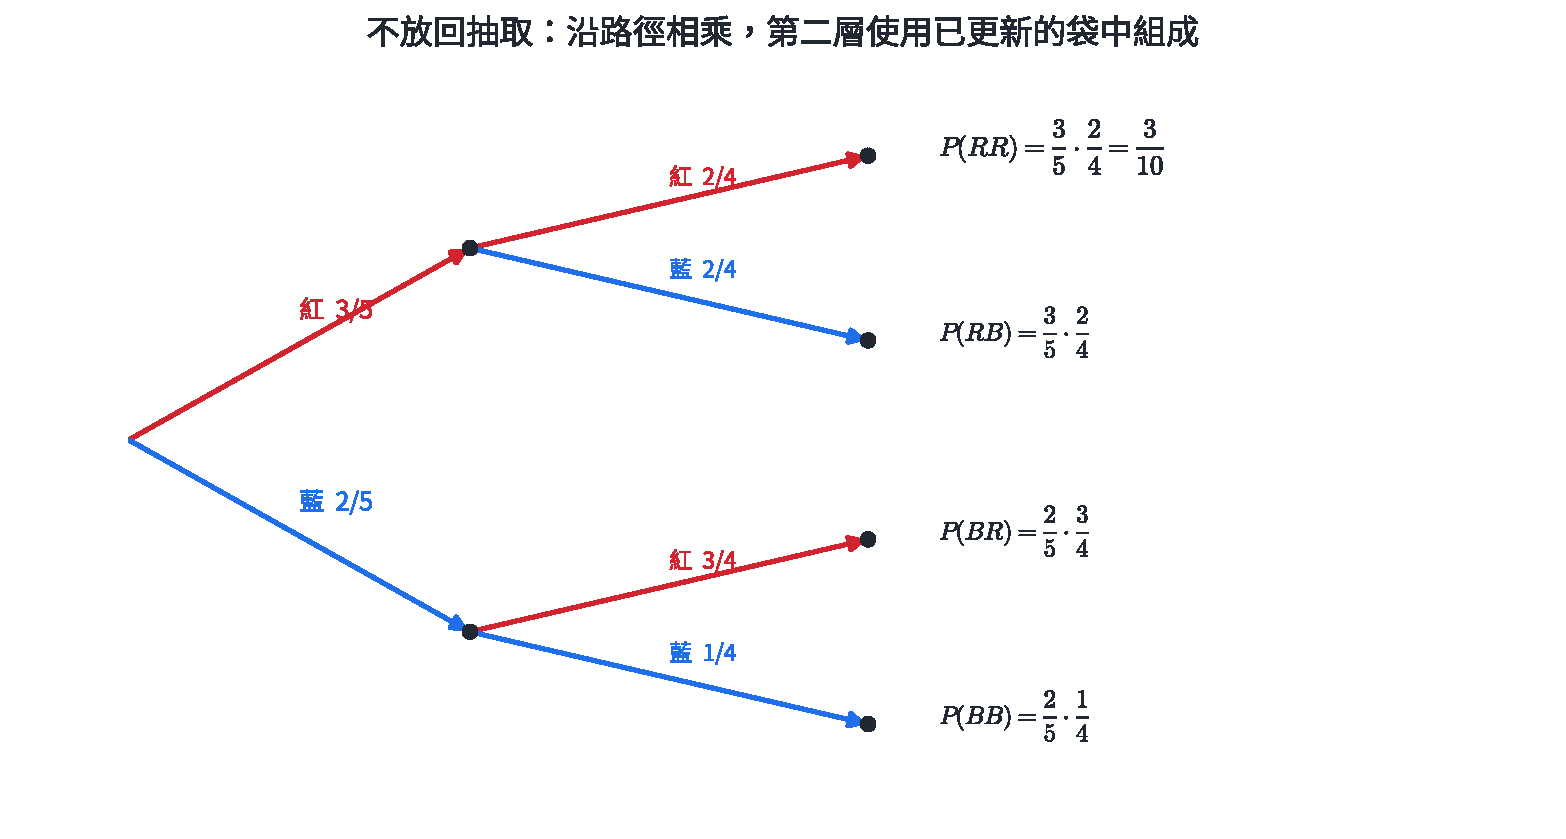
\includegraphics[width=0.9\linewidth,height=\textheight,keepaspectratio,alt={圖 4｜不放回抽球時，第二次的分母與球數已由第一次結果更新；一條路徑的機率沿枝相乘。}]{assets/數A4-3-序列乘法樹.pdf}
\caption{圖 4｜不放回抽球時，第二次的分母與球數已由第一次結果更新；一條路徑的機率沿枝相乘。}
\end{figure}

\begin{HandoutWorkedExample}

\subsection{完整示範｜不放回連取兩球}\label{ux5b8cux6574ux793aux7bc4ux4e0dux653eux56deux9023ux53d6ux5169ux7403}

袋中有 \(3\) 顆紅球、\(2\) 顆藍球，不放回連取兩球。求兩球都是紅球的機率。

令 \(R_1,R_2\) 分別表示第一、二球為紅球：

\[
\begin{aligned}
P(R_1\cap R_2)
&=P(R_1)P(R_2\mid R_1)\\
&=\frac35\cdot\frac24\\
&=\boxed{\frac3{10}}.
\end{aligned}
\]

第一球已取走一顆紅球，因此第二個因子使用剩下 \(4\) 球中的 \(2\) 顆紅球。

\end{HandoutWorkedExample}

\begin{HandoutWorkedExample}

\subsection{完整示範｜三步路徑與指定順序}\label{ux5b8cux6574ux793aux7bc4ux4e09ux6b65ux8defux5f91ux8207ux6307ux5b9aux9806ux5e8f}

袋中有 \(4\) 顆紅球、\(3\) 顆白球、\(2\) 顆藍球，不放回依序取三球。求依序為紅、白、藍的機率。

\[
P(RWB)
=\frac49\cdot\frac38\cdot\frac27
=\frac{24}{504}
=\boxed{\frac1{21}}.
\]

每次分母依序為 \(9,8,7\)；分子依指定顏色的剩餘數量更新。

\end{HandoutWorkedExample}

\subsection{3.2 重複試驗、餘事件與停止規則}\label{ux91cdux8907ux8a66ux9a57ux9918ux4e8bux4ef6ux8207ux505cux6b62ux898fux5247}

當每次試驗獨立且成功率固定為 \(p\)，指定長度為 \(n\) 的成功／失敗序列，其機率是各步因子的乘積。例如前兩次失敗、第三次首次成功：

\[
(1-p)^2p.
\]

恰有 \(k\) 次成功時，先選出成功出現的位置，再乘每一條同型路徑的機率：

\[
P(X=k)=\binom nk p^k(1-p)^{n-k}.
\]

\begin{HandoutWorkedExample}

\subsection{完整示範｜生日碰撞使用餘事件}\label{ux5b8cux6574ux793aux7bc4ux751fux65e5ux78b0ux649eux4f7fux7528ux9918ux4e8bux4ef6}

假設一年 \(365\) 天等可能，忽略閏日，求 \(25\) 人中至少兩人同生日的機率。

直接列舉所有碰撞型態很繁複；餘事件「所有人生日皆不同」只有一條乘法結構：

\[
P(\text{全不同})
=1\cdot\frac{364}{365}\cdot\frac{363}{365}\cdots\frac{341}{365}.
\]

因此

\[
P(\text{至少同生日})
=1-P(\text{全不同})
\approx\boxed{0.5687}.
\]

人數增加時，每一位新成員都要避開更多已占用日期，乘積因此快速下降。

\end{HandoutWorkedExample}

\begin{HandoutWorkedExample}

\subsection{完整示範｜系列賽的停止規則}\label{ux5b8cux6574ux793aux7bc4ux7cfbux5217ux8cfdux7684ux505cux6b62ux898fux5247}

五戰三勝制進行兩局後，甲、乙各勝一局。之後每局甲勝率為 \(0.60\)，各局獨立。求甲贏得系列賽的機率。

接下來最多三局，甲需至少贏兩局。可按三局完整序列計算：

\[
\begin{aligned}
P(\text{甲晉級})
&=\binom32(0.6)^2(0.4)+(0.6)^3\\
&=3(0.36)(0.4)+0.216\\
&=\boxed{0.648}.
\end{aligned}
\]

這個寫法把已提前結束的 \(WW\) 路徑拆成 \(WWW\) 與 \(WWL\) 兩個等價的完整三局結果，總機率保持一致。

\end{HandoutWorkedExample}

\begin{HandoutSelfCheck}

\subsection{分節練習｜乘法法則與路徑}\label{ux5206ux7bc0ux7df4ux7fd2ux4e58ux6cd5ux6cd5ux5247ux8207ux8defux5f91}

\begin{enumerate}
\def\labelenumi{\arabic{enumi}.}
\tightlist
\item
  袋中有 \(5\) 紅、\(3\) 白，不放回連取三球，求依序紅、白、紅的機率。
\item
  \(10\) 支籤中有 \(3\) 支中獎，三人依序不放回各抽一支，求三人都未中獎的機率。
\item
  假設生日在 \(365\) 天等可能，寫出 \(5\) 人中至少兩人同生日的精確機率。
\item
  每次射擊命中率為 \(0.40\) 且各次獨立，求前兩次未中、第三次首次命中的機率。
\item
  每次成功率為 \(0.20\)，獨立進行 \(5\) 次，求恰有 \(2\) 次成功的機率。
\item
  五戰三勝制前兩局戰成 \(1:1\)，之後每局甲勝率 \(0.60\) 且獨立，求甲贏得系列賽的機率。
\end{enumerate}

\textbf{解答}

\begin{enumerate}
\def\labelenumi{\arabic{enumi}.}
\tightlist
\item
  \(\dfrac58\dfrac37\dfrac46=\boxed{\dfrac5{28}}\)。
\item
  \(\dfrac7{10}\dfrac69\dfrac58=\boxed{\dfrac7{24}}\)。
\item
  \(\boxed{1-\dfrac{365\cdot364\cdot363\cdot362\cdot361}{365^5}}\)。
\item
  \((0.60)^2(0.40)=\boxed{0.144}\)。
\item
  \(\binom52(0.2)^2(0.8)^3=\boxed{0.2048}\)。
\item
  \(\binom32(0.6)^2(0.4)+(0.6)^3=\boxed{0.648}\)。
\end{enumerate}

\end{HandoutSelfCheck}

\section{4. 樣本空間分割與全機率公式}\label{ux6a23ux672cux7a7aux9593ux5206ux5272ux8207ux5168ux6a5fux7387ux516cux5f0f}

\subsection{4.1 分割：把所有來源分成互斥且完整的類別}\label{ux5206ux5272ux628aux6240ux6709ux4f86ux6e90ux5206ux6210ux4e92ux65a5ux4e14ux5b8cux6574ux7684ux985eux5225}

事件 \(A_1,A_2,\ldots,A_n\) 稱為樣本空間 \(S\) 的一個分割，需同時滿足：

\[
A_i\cap A_j=\emptyset\quad(i\ne j),
\]

\[
A_1\cup A_2\cup\cdots\cup A_n=S.
\]

若事件 \(B\) 可由不同來源產生，則

\[
B=(B\cap A_1)\cup(B\cap A_2)\cup\cdots\cup(B\cap A_n).
\]

右側各塊互斥，因此機率可相加。再把每一塊用乘法法則改寫，得到全機率公式：

\[
\boxed{
P(B)=\sum_{i=1}^{n}P(A_i)P(B\mid A_i)
}.
\]

這是一個加權平均：\(P(A_i)\) 是第 \(i\) 類在整體中的權重，\(P(B\mid A_i)\) 是該類內部的事件率。

\begin{figure}
\centering
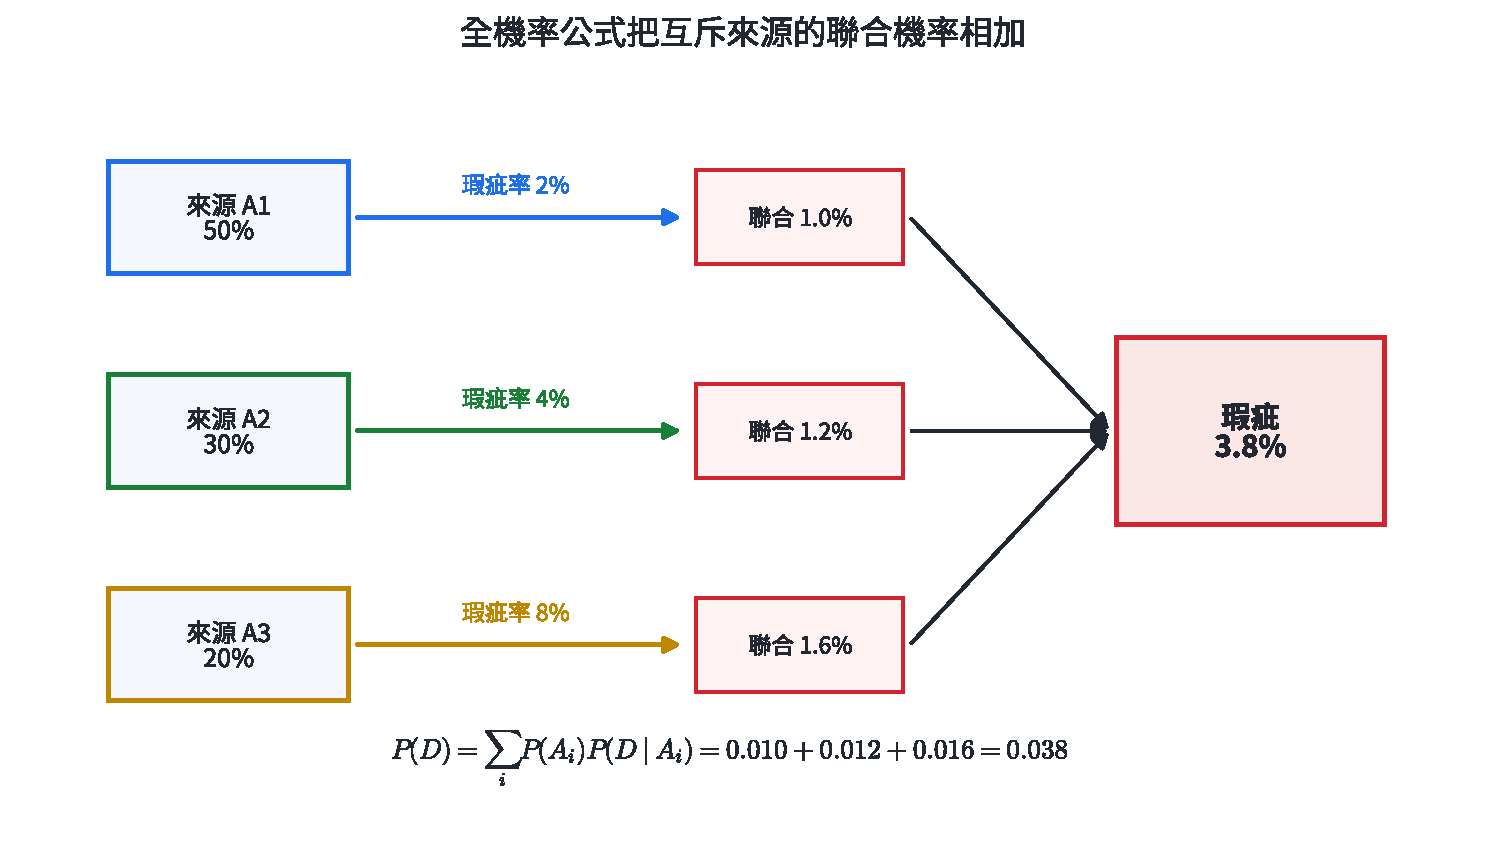
\includegraphics[width=0.92\linewidth,height=\textheight,keepaspectratio,alt={圖 5｜三個來源先各自產生聯合機率，再把通往瑕疵的互斥路徑相加。}]{assets/數A4-3-全機率分割.pdf}
\caption{圖 5｜三個來源先各自產生聯合機率，再把通往瑕疵的互斥路徑相加。}
\end{figure}

\begin{HandoutWorkedExample}

\subsection{完整示範｜三座工廠的整體瑕疵率}\label{ux5b8cux6574ux793aux7bc4ux4e09ux5ea7ux5de5ux5ee0ux7684ux6574ux9ad4ux7455ux75b5ux7387}

產品來源與各自瑕疵率如下：

{\def\LTcaptype{none} % do not increment counter
\begin{longtable}[]{@{}lrr@{}}
\toprule\noalign{}
來源 & 產量比例 & 瑕疵率 \\
\midrule\noalign{}
\endhead
\bottomrule\noalign{}
\endlastfoot
\(A_1\) & \(0.50\) & \(0.02\) \\
\(A_2\) & \(0.30\) & \(0.04\) \\
\(A_3\) & \(0.20\) & \(0.08\) \\
\end{longtable}
}

令 \(D\) 為瑕疵事件。三條通往 \(D\) 的聯合機率為

\[
0.50(0.02)=0.010,
\]

\[
0.30(0.04)=0.012,
\]

\[
0.20(0.08)=0.016.
\]

所以

\[
P(D)=0.010+0.012+0.016=\boxed{0.038}.
\]

整體瑕疵率 \(3.8\%\) 位於三個分組瑕疵率 \(2\%,4\%,8\%\) 之間，符合加權平均的範圍。

\end{HandoutWorkedExample}

\begin{HandoutWorkedExample}

\subsection{完整示範｜天氣狀態與預報結果}\label{ux5b8cux6574ux793aux7bc4ux5929ux6c23ux72c0ux614bux8207ux9810ux5831ux7d50ux679c}

某地明天實際晴天、雨天的機率分別為 \(0.70,0.30\)。晴天時預報為雨的機率為 \(0.10\)；雨天時預報為雨的機率為 \(0.80\)。求預報為雨的機率。

實際天氣形成分割。令 \(F\) 為預報雨：

\[
\begin{aligned}
P(F)
&=P(\text{晴})P(F\mid \text{晴})+P(\text{雨})P(F\mid \text{雨})\\
&=0.70(0.10)+0.30(0.80)\\
&=0.07+0.24\\
&=\boxed{0.31}.
\end{aligned}
\]

預報雨的 \(31\%\) 由「晴天誤報」與「雨天正確預報」兩條互斥路徑組成。

\end{HandoutWorkedExample}

\begin{HandoutWorkedExample}

\subsection{完整示範｜骰子決定選袋}\label{ux5b8cux6574ux793aux7bc4ux9ab0ux5b50ux6c7aux5b9aux9078ux888b}

擲一顆公正骰子：\(1,2,3\) 點選甲袋，\(4,5\) 點選乙袋，\(6\) 點選丙袋。三袋取到紅球的機率依序為 \(1/4,3/5,1/2\)。求最後取到紅球的機率。

選袋機率為 \(1/2,1/3,1/6\)。因此

\[
\begin{aligned}
P(R)
&=\frac12\cdot\frac14
+\frac13\cdot\frac35
+\frac16\cdot\frac12\\
&=\frac{15+24+10}{120}\\
&=\boxed{\frac{49}{120}}.
\end{aligned}
\]

選袋不是等可能時，第一層權重必須依骰子規則決定。

\end{HandoutWorkedExample}

\begin{HandoutSelfCheck}

\subsection{分節練習｜全機率公式}\label{ux5206ux7bc0ux7df4ux7fd2ux5168ux6a5fux7387ux516cux5f0f}

\begin{enumerate}
\def\labelenumi{\arabic{enumi}.}
\tightlist
\item
  甲、乙兩廠產量占 \(0.60,0.40\)，瑕疵率為 \(0.03,0.05\)。求整體瑕疵率。
\item
  某校高一、高二、高三比例為 \(0.35,0.33,0.32\)，參加社團的比例依序為 \(0.80,0.90,0.40\)。求任選一人有參加社團的機率。
\item
  實際晴天、雨天機率為 \(0.70,0.30\)；晴天時預報雨率 \(0.10\)，雨天時預報雨率 \(0.80\)。求預報雨的機率。
\item
  通勤者選公車、火車、自行車的比例為 \(0.50,0.30,0.20\)，各方式遲到率為 \(0.10,0.05,0.20\)。求整體遲到率。
\item
  產品來自甲廠的比例為 \(x\)、乙廠為 \(1-x\)，兩廠瑕疵率為 \(0.02,0.08\)。若整體瑕疵率為 \(0.05\)，求 \(x\)。
\item
  證明全機率公式所得 \(P(B)\) 必位於所有 \(P(B\mid A_i)\) 的最小值與最大值之間。
\end{enumerate}

\textbf{解答}

\begin{enumerate}
\def\labelenumi{\arabic{enumi}.}
\tightlist
\item
  \(0.60(0.03)+0.40(0.05)=\boxed{0.038}\)。
\item
  \(0.35(0.80)+0.33(0.90)+0.32(0.40)=\boxed{0.705}\)。
\item
  \(0.70(0.10)+0.30(0.80)=\boxed{0.31}\)。
\item
  \(0.50(0.10)+0.30(0.05)+0.20(0.20)=\boxed{0.105}\)。
\item
  \(0.02x+0.08(1-x)=0.05\)，解得 \(\boxed{x=0.50}\)。
\item
  設 \(m\le P(B\mid A_i)\le M\)。乘上非負權重 \(P(A_i)\) 後相加，且 \(\sum_iP(A_i)=1\)，得 \(m\le\sum_iP(A_i)P(B\mid A_i)\le M\)。
\end{enumerate}

\end{HandoutSelfCheck}

\section{5. 貝氏定理：由結果更新來源}\label{ux8c9dux6c0fux5b9aux7406ux7531ux7d50ux679cux66f4ux65b0ux4f86ux6e90}

\subsection{5.1 先算聯合機率，再在觀察結果中重新正規化}\label{ux5148ux7b97ux806fux5408ux6a5fux7387ux518dux5728ux89c0ux5bdfux7d50ux679cux4e2dux91cdux65b0ux6b63ux898fux5316}

分割 \(A_1,\ldots,A_n\) 表示可能來源，\(B\) 表示已觀察到的證據。條件機率給出

\[
P(A_i\mid B)=\frac{P(A_i\cap B)}{P(B)}.
\]

分子用乘法法則，分母用全機率公式，即得

\[
\boxed{
P(A_i\mid B)
=\frac{P(A_i)P(B\mid A_i)}
{\sum_{j=1}^{n}P(A_j)P(B\mid A_j)}
}.
\]

\(P(A_i)\) 是觀察前的來源機率；\(P(B\mid A_i)\) 衡量該來源產生目前證據的能力；\(P(A_i\mid B)\) 是觀察後重新分配的來源機率。

\begin{figure}
\centering
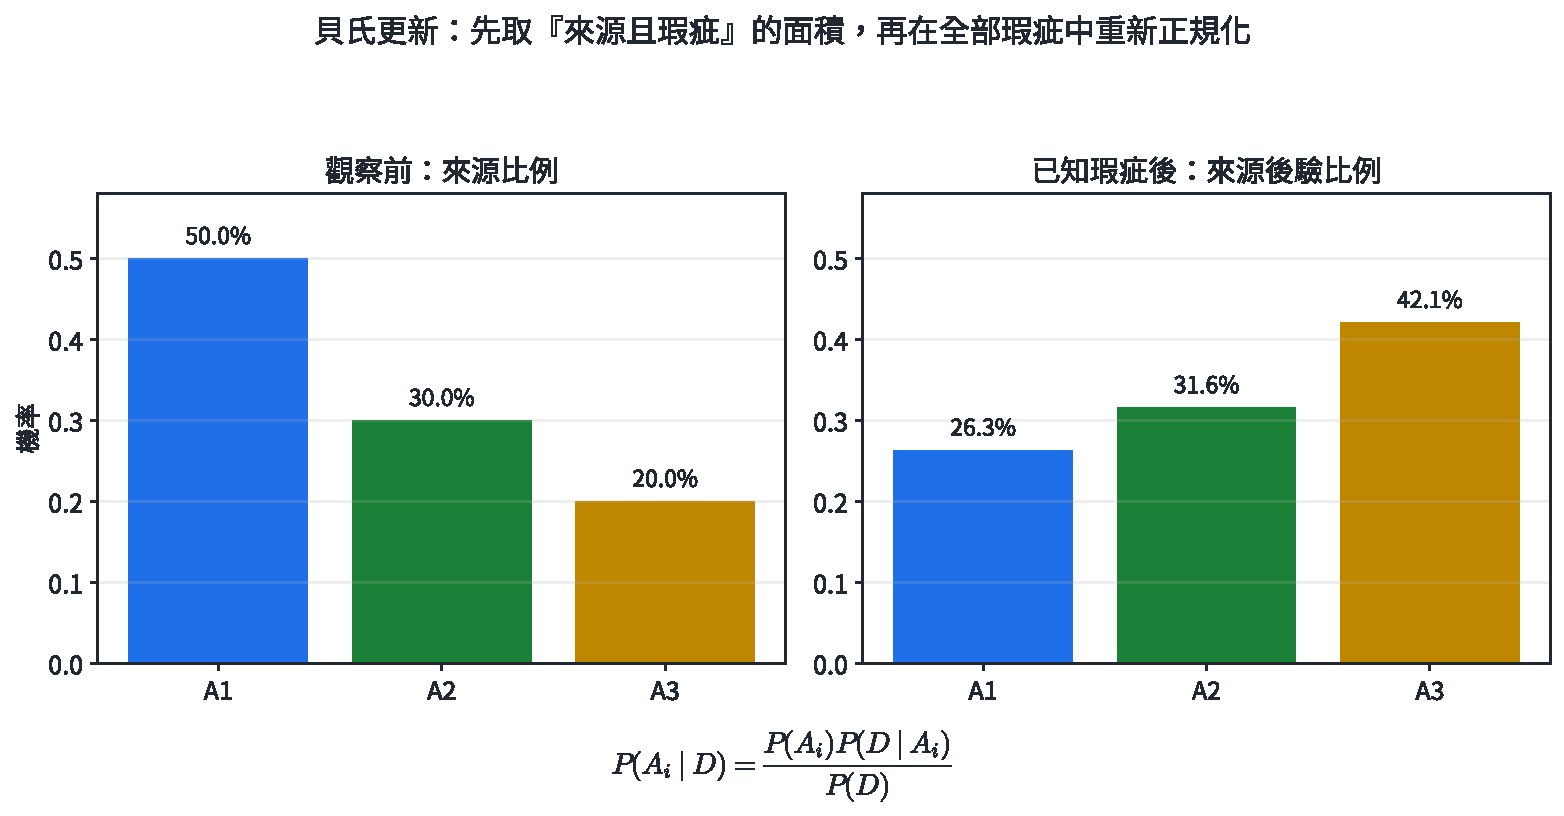
\includegraphics[width=0.88\linewidth,height=\textheight,keepaspectratio,alt={圖 6｜看到瑕疵前以產量比例分配；看到瑕疵後，只在三塊「來源且瑕疵」中重新計算比例。}]{assets/數A4-3-貝氏面積更新.pdf}
\caption{圖 6｜看到瑕疵前以產量比例分配；看到瑕疵後，只在三塊「來源且瑕疵」中重新計算比例。}
\end{figure}

\begin{HandoutWorkedExample}

\subsection{完整示範｜由瑕疵品反推來源工廠}\label{ux5b8cux6574ux793aux7bc4ux7531ux7455ux75b5ux54c1ux53cdux63a8ux4f86ux6e90ux5de5ux5ee0}

沿用上一節資料：三廠產量比例為 \(0.50,0.30,0.20\)，瑕疵率為 \(0.02,0.04,0.08\)。已知抽到瑕疵品，求它來自第三廠的機率。

第三廠且瑕疵的聯合機率為 \(0.20(0.08)=0.016\)；全部瑕疵機率為 \(0.038\)。因此

\[
P(A_3\mid D)
=\frac{0.016}{0.038}
=\frac8{19}
\approx\boxed{0.421}.
\]

第三廠原本只占 \(20\%\)，但瑕疵率最高；觀察到瑕疵後，它的來源比例提升到約 \(42.1\%\)。

\end{HandoutWorkedExample}

\subsection{5.2 檢驗中的基準率、靈敏度與偽陽率}\label{ux6aa2ux9a57ux4e2dux7684ux57faux6e96ux7387ux9748ux654fux5ea6ux8207ux507dux967dux7387}

檢驗問題通常同時包含三種資料：

\begin{itemize}
\tightlist
\item
  盛行率 \(P(D)\)：受測前確實有狀況的比例；
\item
  靈敏度 \(P(+\mid D)\)：有狀況者檢出陽性的比例；
\item
  偽陽率 \(P(+\mid D')\)：沒有狀況者仍呈陽性的比例。
\end{itemize}

陽性後確實有狀況的機率為

\[
P(D\mid+)
=\frac{P(D)P(+\mid D)}
{P(D)P(+\mid D)+P(D')P(+\mid D')}.
\]

\begin{HandoutWorkedExample}

\subsection{完整示範｜用自然頻數解讀快篩陽性}\label{ux5b8cux6574ux793aux7bc4ux7528ux81eaux7136ux983bux6578ux89e3ux8b80ux5febux7be9ux967dux6027}

某狀況盛行率為 \(2\%\)，檢驗靈敏度為 \(90\%\)，偽陽率為 \(5\%\)。求陽性者確實有狀況的機率。

以 \(10{,}000\) 人為共同母體：

\begin{itemize}
\tightlist
\item
  有狀況 \(200\) 人，其中陽性 \(200(0.90)=180\) 人；
\item
  無狀況 \(9{,}800\) 人，其中陽性 \(9{,}800(0.05)=490\) 人。
\end{itemize}

陽性共 \(180+490=670\) 人，因此

\[
P(D\mid+)=\frac{180}{670}
=\frac{18}{67}
\approx\boxed{0.269}.
\]

陽性只是新證據；它需要和受測前的基準率一起解讀。

\end{HandoutWorkedExample}

\begin{figure}
\centering
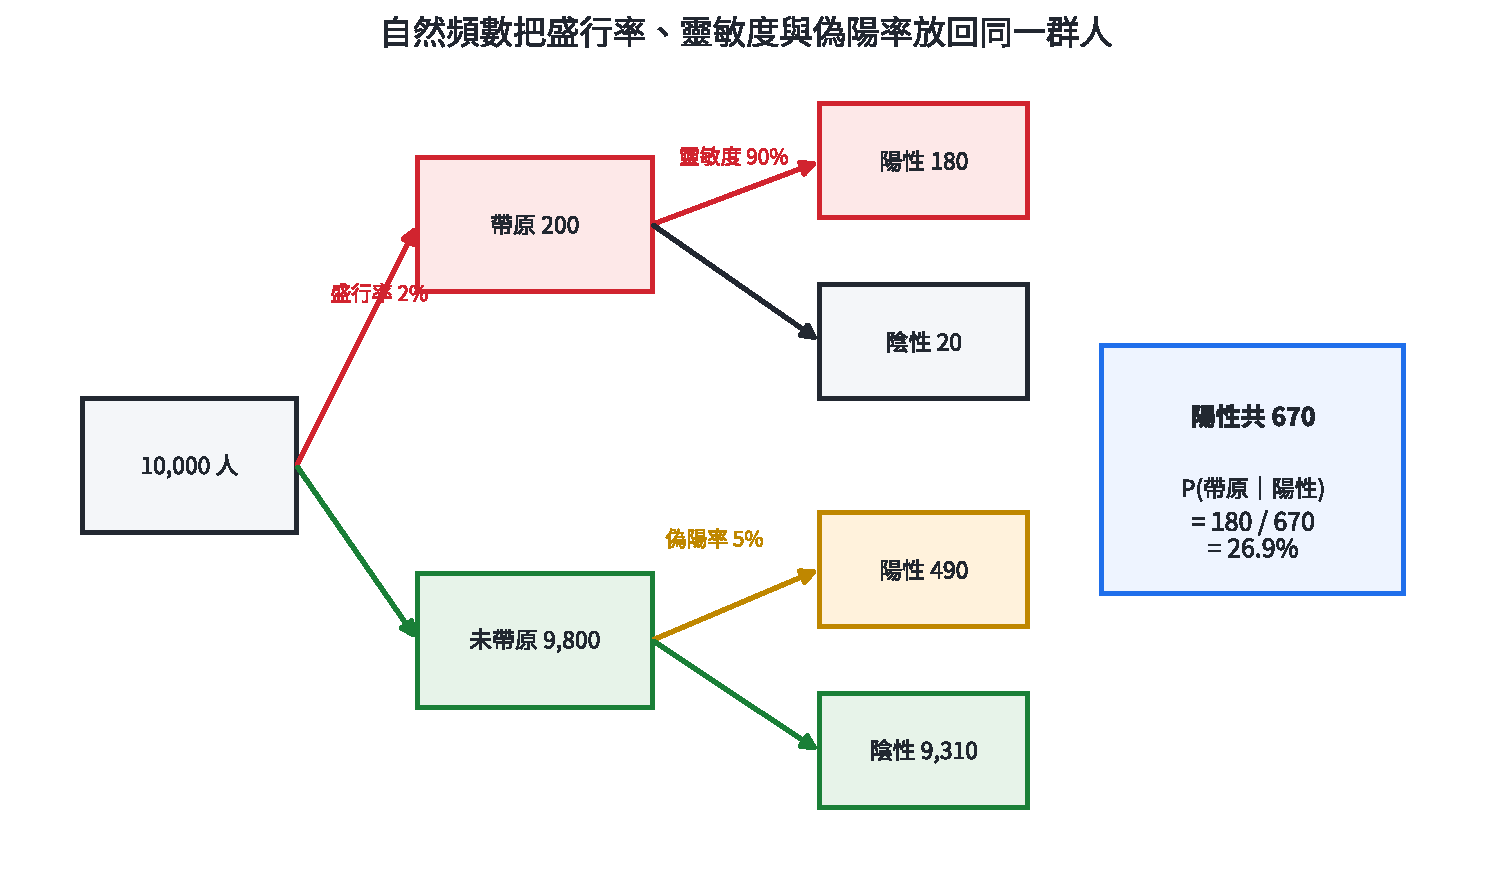
\includegraphics[width=0.92\linewidth,height=\textheight,keepaspectratio,alt={圖 7｜自然頻數把兩種陽性來源放入同一人數尺度，分母 670 可直接由圖讀出。}]{assets/數A4-3-快篩自然頻數.pdf}
\caption{圖 7｜自然頻數把兩種陽性來源放入同一人數尺度，分母 670 可直接由圖讀出。}
\end{figure}

\begin{HandoutWorkedExample}

\subsection{完整示範｜選盒後看到金幣}\label{ux5b8cux6574ux793aux7bc4ux9078ux76d2ux5f8cux770bux5230ux91d1ux5e63}

等機率選一個盒子。甲盒兩格都是金幣；乙盒一格金幣、一格銀幣。再等機率開一格，已知看到金幣，求選到甲盒的機率。

令 \(G\) 為看到金幣：

\[
P(G\mid \text{甲})=1,
\qquad
P(G\mid \text{乙})=\frac12.
\]

\[
P(\text{甲}\mid G)
=\frac{\frac12(1)}{\frac12(1)+\frac12(\frac12)}
=\boxed{\frac23}.
\]

看到金幣後，甲盒的可能性提高，因為甲盒每一格都能產生這項證據。

\end{HandoutWorkedExample}

\begin{HandoutWorkedExample}

\subsection{完整示範｜第一次治療失敗後估計第二次成功}\label{ux5b8cux6574ux793aux7bc4ux7b2cux4e00ux6b21ux6cbbux7642ux5931ux6557ux5f8cux4f30ux8a08ux7b2cux4e8cux6b21ux6210ux529f}

某疾病有兩型：第一型占 \(60\%\)，每次療程成功率 \(75\%\)，各次療程在已知型別下獨立；第二型占 \(40\%\)，此療法成功率為 \(0\)。第一次療程失敗後，求第二次成功的機率。

先用第一次失敗 \(F_1\) 更新型別：

\[
P(I\mid F_1)
=\frac{0.60(0.25)}{0.60(0.25)+0.40(1)}
=\frac{0.15}{0.55}
=\frac3{11}.
\]

第二次只有第一型可能成功，所以

\[
P(S_2\mid F_1)
=P(I\mid F_1)P(S_2\mid I,F_1)
=\frac3{11}\cdot\frac34
=\boxed{\frac9{44}}.
\]

第一次失敗降低了第一型的後驗比例，因此第二次成功率也由受測前的 \(0.60(0.75)=0.45\) 降為約 \(0.205\)。

\end{HandoutWorkedExample}

\begin{HandoutSelfCheck}

\subsection{分節練習｜貝氏更新}\label{ux5206ux7bc0ux7df4ux7fd2ux8c9dux6c0fux66f4ux65b0}

\begin{enumerate}
\def\labelenumi{\arabic{enumi}.}
\tightlist
\item
  產品來自甲、乙廠的比例為 \(0.30,0.70\)，瑕疵率為 \(0.02,0.04\)。已知是瑕疵品，求來自乙廠的機率。
\item
  某狀況盛行率 \(0.10\)，檢驗靈敏度 \(0.95\)，偽陽率 \(0.05\)。求陽性者確實有狀況的機率。
\item
  實際晴天、雨天機率 \(0.70,0.30\)；晴天時預報雨率 \(0.10\)，雨天時預報雨率 \(0.80\)。已知預報雨，求實際下雨的機率。
\item
  等機率選甲、乙盒；甲盒兩枚金幣，乙盒一金一銀。任取一枚後看到金幣，求選到甲盒的機率。
\item
  三供應商供貨比例為 \(0.20,0.30,0.50\)，瑕疵率為 \(0.01,0.02,0.03\)。已知抽到瑕疵品，求來自第三供應商的機率。
\item
  某檢驗靈敏度 \(0.80\)、偽陽率 \(0.10\)。已知陽性者確實有狀況的機率為 \(0.40\)，求受測群體的盛行率。
\end{enumerate}

\textbf{解答}

\begin{enumerate}
\def\labelenumi{\arabic{enumi}.}
\tightlist
\item
  \(\dfrac{0.70(0.04)}{0.30(0.02)+0.70(0.04)}=\dfrac{0.028}{0.034}=\boxed{\dfrac{14}{17}}\)。
\item
  \(\dfrac{0.10(0.95)}{0.10(0.95)+0.90(0.05)}=\dfrac{0.095}{0.140}=\boxed{\dfrac{19}{28}}\)。
\item
  \(\dfrac{0.30(0.80)}{0.70(0.10)+0.30(0.80)}=\boxed{\dfrac{24}{31}}\)。
\item
  \(\dfrac{(1/2)(1)}{(1/2)(1)+(1/2)(1/2)}=\boxed{2/3}\)。
\item
  \(\dfrac{0.50(0.03)}{0.20(0.01)+0.30(0.02)+0.50(0.03)}=\boxed{\dfrac{15}{23}}\)。
\item
  令盛行率為 \(p\)：\(\dfrac{0.8p}{0.8p+0.1(1-p)}=0.4\)，解得 \(\boxed{p=1/13\approx0.0769}\)。
\end{enumerate}

\end{HandoutSelfCheck}

\section{6. 古典、客觀與主觀機率}\label{ux53e4ux5178ux5ba2ux89c0ux8207ux4e3bux89c0ux6a5fux7387}

\subsection{6.1 三種機率敘述的證據來源}\label{ux4e09ux7a2eux6a5fux7387ux6558ux8ff0ux7684ux8b49ux64daux4f86ux6e90}

同一個 \(0\) 到 \(1\) 的數值，可能來自不同證據：

{\def\LTcaptype{none} % do not increment counter
\begin{longtable}[]{@{}
  >{\raggedright\arraybackslash}p{(\linewidth - 6\tabcolsep) * \real{0.2500}}
  >{\raggedright\arraybackslash}p{(\linewidth - 6\tabcolsep) * \real{0.2500}}
  >{\raggedright\arraybackslash}p{(\linewidth - 6\tabcolsep) * \real{0.2500}}
  >{\raggedright\arraybackslash}p{(\linewidth - 6\tabcolsep) * \real{0.2500}}@{}}
\toprule\noalign{}
\begin{minipage}[b]{\linewidth}\raggedright
類型
\end{minipage} & \begin{minipage}[b]{\linewidth}\raggedright
來源
\end{minipage} & \begin{minipage}[b]{\linewidth}\raggedright
例子
\end{minipage} & \begin{minipage}[b]{\linewidth}\raggedright
主要限制
\end{minipage} \\
\midrule\noalign{}
\endhead
\bottomrule\noalign{}
\endlastfoot
古典機率 & 有限且等可能的樣本點 & 公正骰子出現偶數為 \(3/6\) & 等可能假設要成立 \\
客觀／頻率機率 & 重複觀察或歷史資料的相對次數 & 10,000 件中 380 件瑕疵，估計為 \(0.038\) & 母體、時間與測量條件要相近 \\
主觀機率 & 個人依資訊、經驗形成的信念程度 & 專案經理估計如期完成率 \(0.70\) & 需說明依據並接受新證據校正 \\
\end{longtable}
}

三種類型都必須符合機率公理。資料型機率還需檢查抽樣方式、樣本大小、條件是否改變；貝氏更新則提供一套把原先判斷與新證據結合的規則。

\begin{figure}
\centering
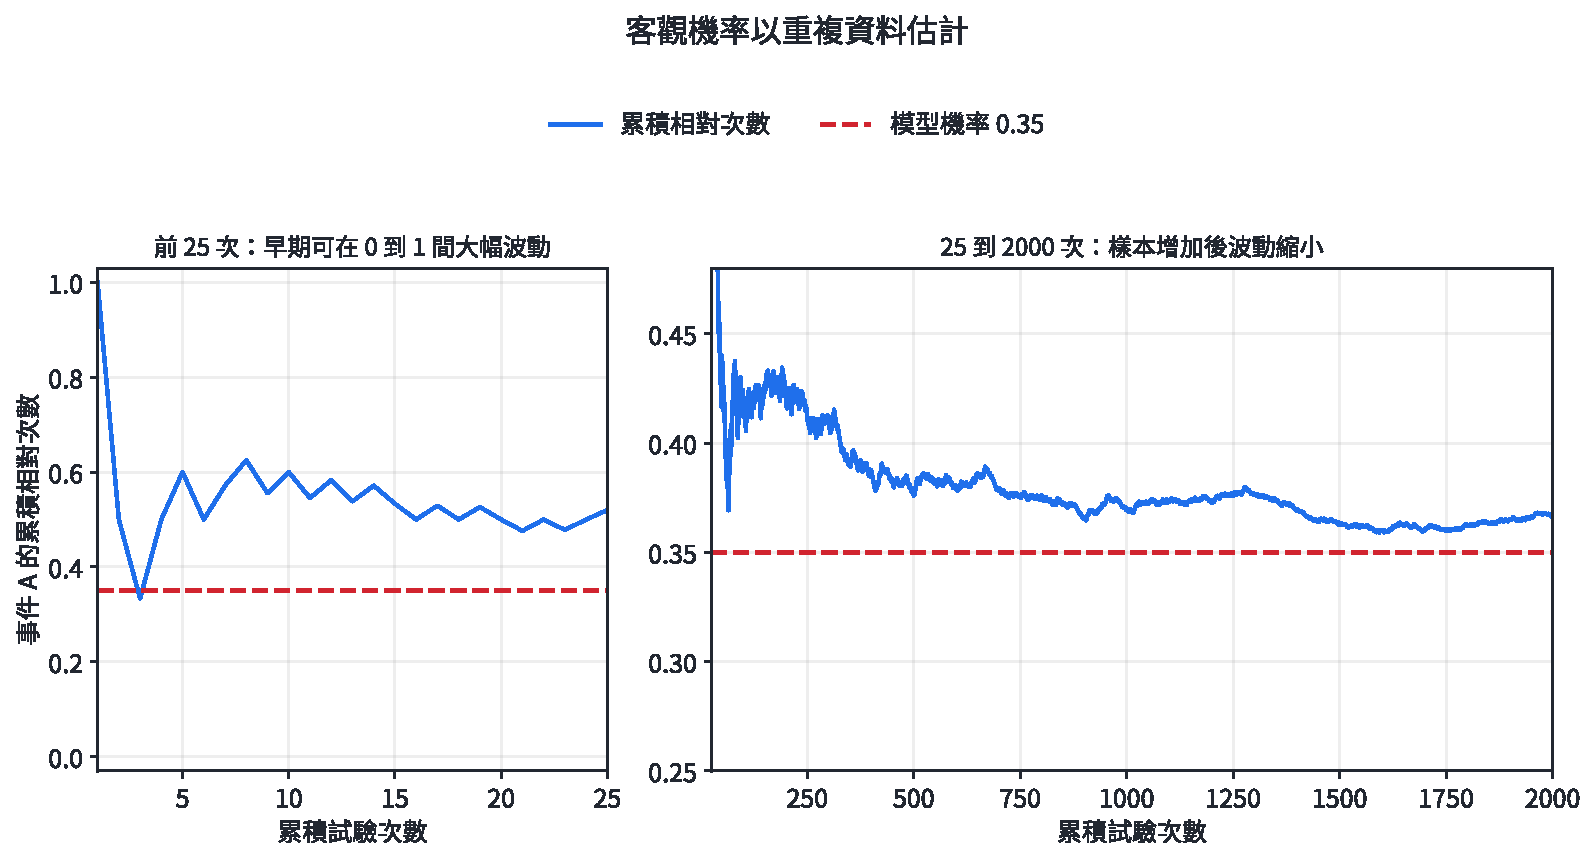
\includegraphics[width=0.88\linewidth,height=\textheight,keepaspectratio,alt={圖 8｜固定模型機率下，累積相對次數仍會波動；試驗數增加時，單次結果對比例的影響逐漸變小。}]{assets/數A4-3-客觀機率收斂.pdf}
\caption{圖 8｜固定模型機率下，累積相對次數仍會波動；試驗數增加時，單次結果對比例的影響逐漸變小。}
\end{figure}

\begin{HandoutWorkedExample}

\subsection{完整示範｜判斷機率敘述的來源}\label{ux5b8cux6574ux793aux7bc4ux5224ux65b7ux6a5fux7387ux6558ux8ff0ux7684ux4f86ux6e90}

判斷下列敘述：

\begin{enumerate}
\def\labelenumi{\arabic{enumi}.}
\tightlist
\item
  公正硬幣連擲三次皆為正面的機率是 \(1/8\)；
\item
  過去 \(5{,}000\) 筆訂單有 \(120\) 筆逾期，據此估計逾期率 \(2.4\%\)；
\item
  工程師依目前進度判斷本週完成的機率為 \(70\%\)。
\end{enumerate}

第 1 項由等可能樣本點計算，是古典機率；第 2 項由相對次數估計，是客觀／頻率機率；第 3 項是依現有資訊形成的主觀機率。第 3 項仍可在取得新進度資料後用條件機率更新。

\end{HandoutWorkedExample}

\begin{HandoutWorkedExample}

\subsection{完整示範｜相同比例與不同資料量}\label{ux5b8cux6574ux793aux7bc4ux76f8ux540cux6bd4ux4f8bux8207ux4e0dux540cux8cc7ux6599ux91cf}

甲資料為 \(100\) 次中成功 \(35\) 次；乙資料為 \(10{,}000\) 次中成功 \(3{,}500\) 次。兩者相對次數都是

\[
\hat p=0.35.
\]

但新增或修正一筆資料時，甲資料的比例變動單位約為 \(1/100=0.01\)，乙資料約為 \(1/10{,}000=0.0001\)。乙資料對單一觀察更不敏感；使用時仍需確認兩批資料的對象與條件是否能代表目前問題。

\end{HandoutWorkedExample}

\begin{HandoutSelfCheck}

\subsection{分節練習｜機率來源與資料判讀}\label{ux5206ux7bc0ux7df4ux7fd2ux6a5fux7387ux4f86ux6e90ux8207ux8cc7ux6599ux5224ux8b80}

\begin{enumerate}
\def\labelenumi{\arabic{enumi}.}
\tightlist
\item
  判斷下列為古典、客觀或主觀機率：公正骰子出現 6 點為 \(1/6\)；過去千件貨物有 \(18\) 件破損；教練估計球隊明天勝率 \(0.65\)。
\item
  某人說明天下雨機率 \(0.40\)、不下雨機率 \(0.70\)。檢查是否符合機率性質。
\item
  某骰子擲 \(200\) 次，各點次數為 \(28,31,37,35,39,30\)。用客觀機率估計下一次出現偶數點的機率。
\item
  甲樣本 \(50\) 次中成功 \(20\) 次，乙樣本 \(5{,}000\) 次中成功 \(2{,}000\) 次。比較兩個點估計與單筆資料對比例的影響。
\item
  原先估計設備故障率 \(0.05\)；取得新環境條件 \(E\) 後，已知 \(P(E\mid \text{故障})=0.60\)、\(P(E\mid \text{正常})=0.10\)。求看見 \(E\) 後的故障機率。
\end{enumerate}

\textbf{解答}

\begin{enumerate}
\def\labelenumi{\arabic{enumi}.}
\tightlist
\item
  依序為 \(\boxed{\text{古典、客觀、主觀}}\)。
\item
  兩事件互為餘事件，機率應相加為 \(1\)；\(0.40+0.70=1.10\)，所以資料不一致。
\item
  偶數次數為 \(31+35+30=96\)，估計為 \(\boxed{96/200=0.48}\)。
\item
  點估計都為 \(0.40\)；單筆資料造成的比例變動尺度分別約為 \(1/50=0.02\) 與 \(1/5000=0.0002\)。
\item
  \(\dfrac{0.05(0.60)}{0.05(0.60)+0.95(0.10)}=\dfrac{0.03}{0.125}=\boxed{0.24}\)。
\end{enumerate}

\end{HandoutSelfCheck}

\section{7. 核心整理}\label{ux6838ux5fc3ux6574ux7406}

\subsection{條件、乘法與獨立}\label{ux689dux4ef6ux4e58ux6cd5ux8207ux7368ux7acb}

\[
P(B\mid A)=\frac{P(A\cap B)}{P(A)},
\qquad P(A)>0,
\]

\[
P(A\cap B)=P(A)P(B\mid A),
\]

\[
A,B\text{ 獨立}
\quad\Longleftrightarrow\quad
P(A\cap B)=P(A)P(B).
\]

\subsection{分割、全機率與貝氏更新}\label{ux5206ux5272ux5168ux6a5fux7387ux8207ux8c9dux6c0fux66f4ux65b0}

若 \(A_1,\ldots,A_n\) 為樣本空間分割，則

\[
P(B)=\sum_{i=1}^{n}P(A_i)P(B\mid A_i),
\]

\[
P(A_i\mid B)
=\frac{P(A_i)P(B\mid A_i)}
{\sum_jP(A_j)P(B\mid A_j)}.
\]

條件機率先決定目前分母；乘法法則算一條路徑；全機率公式加總所有互斥路徑；貝氏定理把某一路徑在全部觀察結果中的比例取出。

\section{8. 章末分層題}\label{ux7ae0ux672bux5206ux5c64ux984c}

\subsection{基礎題}\label{ux57faux790eux984c}

\begin{enumerate}
\def\labelenumi{\arabic{enumi}.}
\item
  已知 \(P(A)=0.54\)、\(P(B)=0.43\)、\(P(A\cap B)=0.25\)。求 \(P(A\cup B)\) 與 \(P(A'\cap B')\)。
\item
  某年級有 \(240\) 人，其中修讀課程 \(A\) 的有 \(150\) 人，修讀課程 \(B\) 的有 \(120\) 人，兩門都修的有 \(90\) 人。隨機選一人，求 \(P(B\mid A)\)、\(P(A\mid B)\) 與 \(P(A'\mid B)\)。
\item
  擲兩顆公平六面骰。已知點數和為 \(10\)，求第一顆點數大於第二顆的條件機率。
\item
  已知 \(P(A)=0.40\)、\(P(B)=0.50\)、\(P(A\cup B)=0.70\)。判斷 \(A,B\) 是否獨立，並求 \(P(A'\cap B')\)。
\end{enumerate}

\subsection{熟練題}\label{ux719fux7df4ux984c}

\begin{enumerate}
\def\labelenumi{\arabic{enumi}.}
\setcounter{enumi}{4}
\item
  兩部裝置獨立運作，正常率分別為 \(0.95\) 與 \(0.90\)。求兩部都正常、至少一部正常、恰有一部正常的機率。
\item
  三位選手獨立命中目標的機率依序為 \(0.70,0.60,0.80\)。求三人都命中、恰有兩人命中、至少一人命中的機率。
\item
  袋中有 \(6\) 顆紅球與 \(4\) 顆白球，不放回依序取三球。求顏色依序為紅、白、紅的機率。
\item
  假設一年有 \(365\) 天，且每人的生日在各日等可能並彼此獨立。求 \(20\) 人中至少兩人同生日的機率，答案可用乘積表示並取至小數第四位。
\end{enumerate}

\subsection{應用題}\label{ux61c9ux7528ux984c}

\begin{enumerate}
\def\labelenumi{\arabic{enumi}.}
\setcounter{enumi}{8}
\item
  某零件分別由甲、乙、丙三條產線生產，產量比例為 \(0.50,0.30,0.20\)，瑕疵率依序為 \(0.01,0.03,0.06\)。求隨機抽到瑕疵品的機率。
\item
  承第 9 題，已知抽到的是瑕疵品，求它來自丙線的機率。
\item
  某狀況在受測群體中的盛行率為 \(0.04\)。檢驗靈敏度為 \(0.92\)，特異度為 \(0.95\)。求隨機一人檢驗呈陽性的機率，以及陽性者確實有此狀況的機率。
\item
  某項製程先觀察 \(600\) 次，成功 \(210\) 次；之後在相同條件下再觀察 \(400\) 次，成功 \(160\) 次。分別求第一批與合併資料的成功相對次數，並比較新增資料前後的估計。
\end{enumerate}

\subsection{跨節整合題}\label{ux8de8ux7bc0ux6574ux5408ux984c}

\begin{enumerate}
\def\labelenumi{\arabic{enumi}.}
\setcounter{enumi}{12}
\tightlist
\item
  甲、乙兩個主系統獨立故障，故障率分別為 \(0.10\) 與 \(0.20\)。兩者都故障時，備援系統會啟動，且備援成功率為 \(0.90\)。
\end{enumerate}

\begin{enumerate}
\def\labelenumi{(\arabic{enumi})}
\item
  已知至少一個主系統故障，求兩個主系統都故障的機率。
\item
  求整體系統仍能工作的機率。
\end{enumerate}

\begin{enumerate}
\def\labelenumi{\arabic{enumi}.}
\setcounter{enumi}{13}
\item
  一批貨先以機率 \(0.30\) 選甲廠、以機率 \(0.70\) 選乙廠。甲、乙兩廠產品瑕疵率分別為 \(0.02,0.05\)。選定工廠後，從該廠抽兩件；在工廠條件固定時，兩件是否瑕疵相互獨立。已知兩件都是瑕疵品，求這批貨來自乙廠的機率。
\item
  某狀況的盛行率為 \(0.02\)。同一人接受兩次檢驗；在實際狀況固定時，兩次結果條件獨立。每次檢驗的靈敏度為 \(0.90\)、偽陽率為 \(0.05\)。已知兩次結果皆為陽性，求此人確實有狀況的機率。
\item
  某匿名調查以機率 \(0.75\) 顯示問題「你每天使用某服務超過兩小時嗎」，以機率 \(0.25\) 顯示其相反問題「你每天使用某服務不超過兩小時嗎」；受訪者只回答畫面上的問題，畫面種類不被記錄。大量樣本中回答「是」的比例為 \(0.65\)。
\end{enumerate}

\begin{enumerate}
\def\labelenumi{(\arabic{enumi})}
\item
  估計每天使用超過兩小時者的比例。
\item
  隨機查看一筆回答「是」的紀錄，求該人每天使用超過兩小時的機率。
\end{enumerate}

\section{9. 章末題完整解析}\label{ux7ae0ux672bux984cux5b8cux6574ux89e3ux6790}

\subsection{第 1 題}\label{ux7b2c-1-ux984c}

加法公式給出

\[
P(A\cup B)=P(A)+P(B)-P(A\cap B)
=0.54+0.43-0.25
=\boxed{0.72}.
\]

\(A'\cap B'\) 表示兩事件都未發生，是 \(A\cup B\) 的餘事件，因此

\[
P(A'\cap B')=1-P(A\cup B)=\boxed{0.28}.
\]

\subsection{第 2 題}\label{ux7b2c-2-ux984c}

把修讀 \(A\) 視為新的樣本空間，其中同時修讀 \(B\) 的有 \(90\) 人：

\[
P(B\mid A)=\frac{90}{150}=\boxed{0.60}.
\]

把修讀 \(B\) 視為新的樣本空間：

\[
P(A\mid B)=\frac{90}{120}=\boxed{0.75}.
\]

在修讀 \(B\) 的 \(120\) 人中，有 \(120-90=30\) 人未修讀 \(A\)，所以

\[
P(A'\mid B)=\frac{30}{120}=\boxed{0.25}.
\]

三個答案都使用各自條件事件的人數作分母。

\subsection{第 3 題}\label{ux7b2c-3-ux984c}

在「點數和為 \(10\)」的條件下，等可能結果只有

\[
(4,6),\ (5,5),\ (6,4).
\]

第一顆大於第二顆只發生在 \((6,4)\)，所以

\[
P(\text{第一顆}>\text{第二顆}\mid\text{和為 }10)
=\boxed{\frac13}.
\]

\subsection{第 4 題}\label{ux7b2c-4-ux984c}

由加法公式反求交集：

\[
P(A\cap B)=0.40+0.50-0.70=0.20.
\]

同時

\[
P(A)P(B)=0.40(0.50)=0.20,
\]

因此 \(P(A\cap B)=P(A)P(B)\)，\(A,B\) 獨立。兩事件都未發生的機率為

\[
P(A'\cap B')=1-P(A\cup B)=\boxed{0.30}.
\]

也可由獨立事件的餘事件仍獨立，算得 \(0.60(0.50)=0.30\)。

\subsection{第 5 題}\label{ux7b2c-5-ux984c}

令兩部裝置正常事件為 \(N_1,N_2\)。獨立性給出

\[
P(N_1\cap N_2)=0.95(0.90)=\boxed{0.855}.
\]

至少一部正常的餘事件是兩部都故障：

\[
P(N_1\cup N_2)=1-(0.05)(0.10)=\boxed{0.995}.
\]

恰有一部正常包含兩條互斥路徑：

\[
P(N_1\cap N_2')+P(N_1'\cap N_2)
=0.95(0.10)+0.05(0.90)
=\boxed{0.140}.
\]

\subsection{第 6 題}\label{ux7b2c-6-ux984c}

三人都命中的機率為

\[
0.70(0.60)(0.80)=\boxed{0.336}.
\]

恰有兩人命中包含第三人失手、第二人失手、第一人失手三條互斥路徑：

\[
\begin{aligned}
P(\text{恰有兩人命中})
&=0.70(0.60)(0.20)\\
&\quad+0.70(0.40)(0.80)\\
&\quad+0.30(0.60)(0.80)\\
&=0.084+0.224+0.144\\
&=\boxed{0.452}.
\end{aligned}
\]

至少一人命中的餘事件是三人都失手：

\[
P(\text{至少一人命中})
=1-0.30(0.40)(0.20)
=\boxed{0.976}.
\]

\subsection{第 7 題}\label{ux7b2c-7-ux984c}

不放回抽取會改變每一步的分母與分子。沿著紅、白、紅的路徑相乘：

\[
P(R_1W_2R_3)
=\frac6{10}\cdot\frac4{9}\cdot\frac5{8}
=\boxed{\frac16}.
\]

第二次取走一顆白球，因此第三次袋中仍有 \(5\) 顆紅球與 \(8\) 顆球。

\subsection{第 8 題}\label{ux7b2c-8-ux984c}

先算 \(20\) 人生日全都不同。第一人的生日任意；之後每一人要避開先前出現的日期：

\[
P(\text{全不同})
=\frac{365}{365}\cdot\frac{364}{365}\cdots\frac{346}{365}.
\]

因此

\[
\begin{aligned}
P(\text{至少兩人同生日})
&=1-P(\text{全不同})\\
&=1-\frac{365\cdot364\cdots346}{365^{20}}\\
&\approx\boxed{0.4114}.
\end{aligned}
\]

事件「至少有一組相同」包含許多重疊情形，使用餘事件可一次涵蓋它們。

\subsection{第 9 題}\label{ux7b2c-9-ux984c}

以 \(D\) 表示瑕疵。三條產線形成樣本空間分割，依全機率公式

\[
\begin{aligned}
P(D)
&=0.50(0.01)+0.30(0.03)+0.20(0.06)\\
&=0.005+0.009+0.012\\
&=\boxed{0.026}.
\end{aligned}
\]

三項分別表示「來自該產線且為瑕疵品」的聯合機率。

\subsection{第 10 題}\label{ux7b2c-10-ux984c}

丙線且瑕疵的機率已在第 9 題算得 \(0.20(0.06)=0.012\)。在全部瑕疵品中取其比例：

\[
P(\text{丙}\mid D)
=\frac{0.012}{0.026}
=\boxed{\frac6{13}\approx0.4615}.
\]

丙線只占總產量兩成，但較高的瑕疵率使它占全部瑕疵品約四成六。

\subsection{第 11 題}\label{ux7b2c-11-ux984c}

令 \(C\) 表示確實有狀況，\(+\) 表示陽性。特異度 \(0.95\) 對應偽陽率

\[
P(+\mid C')=1-0.95=0.05.
\]

陽性可能來自真陽性或偽陽性：

\[
\begin{aligned}
P(+)
&=P(C)P(+\mid C)+P(C')P(+\mid C')\\
&=0.04(0.92)+0.96(0.05)\\
&=0.0368+0.048\\
&=\boxed{0.0848}.
\end{aligned}
\]

更新後的機率為

\[
P(C\mid +)
=\frac{0.04(0.92)}{0.0848}
=\frac{0.0368}{0.0848}
=\boxed{\frac{23}{53}\approx0.4340}.
\]

在 \(10{,}000\) 人的自然頻數中，約有 \(368\) 位真陽性、\(480\) 位偽陽性；陽性共 \(848\) 人，其中 \(368/848=23/53\) 確實有狀況。

\subsection{第 12 題}\label{ux7b2c-12-ux984c}

第一批的成功相對次數為

\[
\hat p_1=\frac{210}{600}=\boxed{0.35}.
\]

合併後共有 \(600+400=1{,}000\) 次、成功 \(210+160=370\) 次：

\[
\hat p=\frac{370}{1000}=\boxed{0.37}.
\]

第二批的成功比例為 \(160/400=0.40\)，高於第一批的 \(0.35\)，所以合併估計向上移到 \(0.37\)。合併值是依兩批樣本數加權的結果：

\[
0.37=\frac{600}{1000}(0.35)+\frac{400}{1000}(0.40).
\]

\subsection{第 13 題}\label{ux7b2c-13-ux984c}

令 \(F_A,F_B\) 表示甲、乙主系統故障。由獨立性，

\[
P(F_A\cap F_B)=0.10(0.20)=0.02.
\]

至少一個主系統故障的機率為

\[
P(F_A\cup F_B)=1-P(F_A'\cap F_B')
=1-0.90(0.80)=0.28.
\]

所以

\[
P(F_A\cap F_B\mid F_A\cup F_B)
=\frac{0.02}{0.28}
=\boxed{\frac1{14}}.
\]

整體系統失效需要三件事依序成立：兩個主系統都故障，且備援也失敗。備援失敗率為 \(0.10\)，因此

\[
P(\text{整體失效})=0.10(0.20)(0.10)=0.002.
\]

整體仍能工作的機率為

\[
P(\text{整體工作})=1-0.002=\boxed{0.998}.
\]

\subsection{第 14 題}\label{ux7b2c-14-ux984c}

令 \(A,B\) 表示選到甲、乙廠，\(D_1,D_2\) 表示兩件皆為瑕疵的各次事件。在工廠固定的條件下使用條件獨立性：

\[
P(D_1\cap D_2\mid A)=0.02^2,
\qquad
P(D_1\cap D_2\mid B)=0.05^2.
\]

兩件皆瑕疵的總機率為

\[
P(D_1\cap D_2)
=0.30(0.02)^2+0.70(0.05)^2
=0.00012+0.00175
=0.00187.
\]

因此

\[
\begin{aligned}
P(B\mid D_1\cap D_2)
&=\frac{0.70(0.05)^2}{0.00187}\\
&=\boxed{\frac{175}{187}\approx0.9358}.
\end{aligned}
\]

兩次瑕疵提供了比單次更強的來源證據，因此後驗機率集中到瑕疵率較高的乙廠。

\subsection{第 15 題}\label{ux7b2c-15-ux984c}

令 \(C\) 表示確實有狀況，\(++\) 表示兩次皆陽性。題目給定在 \(C\) 或 \(C'\) 固定後，兩次結果條件獨立，所以

\[
P(++\mid C)=0.90^2,
\qquad
P(++\mid C')=0.05^2.
\]

兩次皆陽性的總機率為

\[
P(++)=0.02(0.90)^2+0.98(0.05)^2
=0.0162+0.00245
=0.01865.
\]

因此

\[
\begin{aligned}
P(C\mid ++)
&=\frac{0.02(0.90)^2}{0.01865}\\
&=\boxed{\frac{324}{373}\approx0.8686}.
\end{aligned}
\]

條件獨立性是平方兩個條件機率的依據；若兩次檢驗共用同一項系統性誤差，需以實際聯合機率替代平方模型。

\subsection{第 16 題}\label{ux7b2c-16-ux984c}

令 \(U\) 表示每天使用超過兩小時，\(p=P(U)\)；令 \(Q\) 表示畫面顯示原問題，\(Q'\) 表示顯示相反問題，\(Y\) 表示回答「是」。兩條會產生「是」的路徑為

\begin{itemize}
\tightlist
\item
  顯示原問題且受訪者屬於 \(U\)；
\item
  顯示相反問題且受訪者屬於 \(U'\)。
\end{itemize}

因此

\[
\begin{aligned}
P(Y)
&=P(Q)P(U)+P(Q')P(U')\\
&=0.75p+0.25(1-p)\\
&=0.25+0.50p.
\end{aligned}
\]

由觀察比例 \(P(Y)=0.65\)，得到

\[
0.25+0.50p=0.65
\quad\Longrightarrow\quad
p=\boxed{0.80}.
\]

回答「是」且實際屬於 \(U\) 的聯合機率為

\[
P(Q\cap U)=0.75(0.80)=0.60.
\]

所以

\[
P(U\mid Y)
=\frac{0.60}{0.65}
=\boxed{\frac{12}{13}\approx0.9231}.
\]

個別紀錄仍無法直接辨認受訪者看到哪個問題；大量樣本的回答比例則可透過全機率公式反推出群體比例。


\end{document}
